\clearpage
\chapter{Study Guide 4}

\section{Clustering}
\horizontalline{0}{0}

\begin{center}
    \large{\textbf{Study Guide Instructions}}
\end{center}

\horizontalline{-1}{0}

\begin{itemize}
    \item Submit your work in Gradescope as a PDF - you will identify where your “questions are.”
    \item Identify the question number as you submit.  Since we grade "blind" if the questions are NOT identified, the work WILL NOT BE GRADED and a 0 will be recorded. Always leave enough time to 
    identify the questions when submitting.
    \item One section per page (if a page or less) - We prefer to grade the main solution in a single page, extra work can be included on the following page.
    \item Long instructions may be removed to fit on a single page.
    \item \textbf{Do not start a new question in the middle of a page.}
    \item Solutions to book questions are provided for reference.
    \item You may NOT submit given solutions - this includes minor modifications - as your own.
    \item Solutions that do not show individual engagement with the solutions will be marked as no credit and can be considered a violation of honor code.
    \item If you use the given solutions you must reference or explain how you used them, in particular...
\end{itemize}

\horizontalline{-1}{0}

\begin{center}
    \large{\textbf{Method Selection}}
\end{center}

\horizontalline{-1}{0}

\textbf{For full credit,  EACH book exercise in the Study Guides must use one or more of the following methods and FOR EACH QUESTION.  Identify the number the method by number to ensure full credit.}

\begin{itemize}
    \item \textbf{Method 1} - Provide original examples which demonstrate the ideas of the exercise in addition to your solution.
    \item \textbf{Method 2} - Include and discuss the specific topics needed from the chapter and how they relate to the question.
    \item \textbf{Method 3} - Include original Python code, of reasonable length (as screenshot or text)  to show how the topic or concept was explored.
    \item \textbf{Method 4} - Expand the given solution in a significant way, with additional steps and comments. All steps are justified. This is a good method for a proof for which you are only given a basic outline.
    \item \textbf{Method 5} - Attempt the exercise without looking at the solution and then the solution is used to check work. Words are used to describe the results.
    \item \textbf{Method 6} - Provide an analysis of the strategies used to understand the exercise, describing in detail what was challenging, who helped you or what resources were used. The process of understanding is
    described.
\end{itemize}

% Problem 1
\begin{problem}{Problem 1}
    \begin{statement}{Problem Statement}
        Describe the K-Means algorithm in your own words to someone who has never heard of it. Explain each step.
    \end{statement}

    \begin{highlight}[Solution]
        \subsubsection*{Overview}

        The $k$-means algorithm is an algorithm that helps group or `cluster' vectors together based off of their distances from one another. The algorithm works with a fixed number of vectors usually 
        represented with $N$. These vectors are of an arbitrary size, lets call the size of the vectors $n$. The goal of this algorithm is to cluster the vectors in question into $k$ groups where they
        are being clustered together based off of their similarities between one another. Lets dive into this algorithm with a little more detail. \vspace*{1em}

        \subsubsection*{Initialization}

        Initially, when the $k$-means algorithm is going to be run, the programmer must choose the number of clusters (this number is represented with $k$) that they wish their vectors are to be grouped
        in. The algorithm then chooses an arbitrary starting point called the `centroid' for each cluster. These centroids are usually picked at random. \vspace*{1em}

        \subsubsection*{Calculation}

        Once the number of centroids has been chosen for the given data set, we then calculate the distance for a given data point with each centroid. For each individual data point in the data set, a distance
        calculation is performed to determine what is the smallest distance between the given data point and the centroids. The centroid that has the smallest distance between the given data set is the centroid
        that the data point will be assigned to. \vspace*{1em}

        \subsubsection*{Centroid Update}

        After each iteration of assigning a new data point to a centroid, we calculate the `mean' of these data points and update the centroid location for that specific cluster. Essentially, we are pinpointing
        the new center of the centroid by finding the optimal location of it by finding the average of the co-ordinates of each data point for a given cluster. \vspace*{1em}

        \subsubsection*{Completion}

        After the calculation and centroid update step has been completed for every data point in the data set, we call this convergence meaning that the data points have been correctly assigned to their
        correct centroid and the centroid is in the optimal location for all data sets assigned to it. At this point, the algorithm has finished running and we have successfully clustered all of our data points
        in the given data set. \vspace*{1em}

        \subsubsection*{Summary}

        Overall, the $k$-means algorithm is a very efficient way to group data points in a data set together based off of similar characteristics. Initially, the centroid location is randomly positioned within
        the data set and it is constantly updated based off of the mean of the data that it is assigned to. After this process repeats multiple times, we end up with a clustering of data where the data in the data
        set usually share some common characteristic with one another.
    \end{highlight}
\end{problem}

% Problem 1 Summary
\begin{summary}{Problem 1 Summary}
    \begin{statement}{Procedure}
        \begin{itemize}
            \item Answer the prompts with a concise summary of the $k$-means algorithm
        \end{itemize}
    \end{statement}
    \begin{statement}{Key Concepts}
        \begin{itemize}
            \item $k$-means is algorithm that is used in clustering to group data points together based off of similar characteristics
            \item $k$-means first finds a spot for the centroids in the algorithm to be placed
            \item $k$-means then calculates the distance between the centroid and each of its data points to determine the smallest distance between remaining data points
            \item $k$-means then updates the location of the centroid based off the mean distance between data points that have been assigned to the centroid
            \item $k$-means then is complete when the centroid is placed in the lowest average distance between data points for a given cluster
        \end{itemize}
    \end{statement}
    \begin{statement}{Variations}
        \begin{itemize}
            \item We could be asked to summarize a different process in linear algebra
            \begin{itemize}
                \item We then would have to talk about aspects that pertain to that specific process
            \end{itemize}
        \end{itemize}
    \end{statement}
\end{summary}

% Problem 2
\begin{problem}{Problem 2}
    \begin{statement}{Problem Statement}
        Select one page or section of Chapter One of VMLS to annotate. Include a screenshot of your annotation here. (not example 4.4.1 since that is the next question)
    \end{statement}

    For annotations this week, I have chosen to annotate section 4.2 of VMLS. The annotations for this problem can be seen on the following page.

    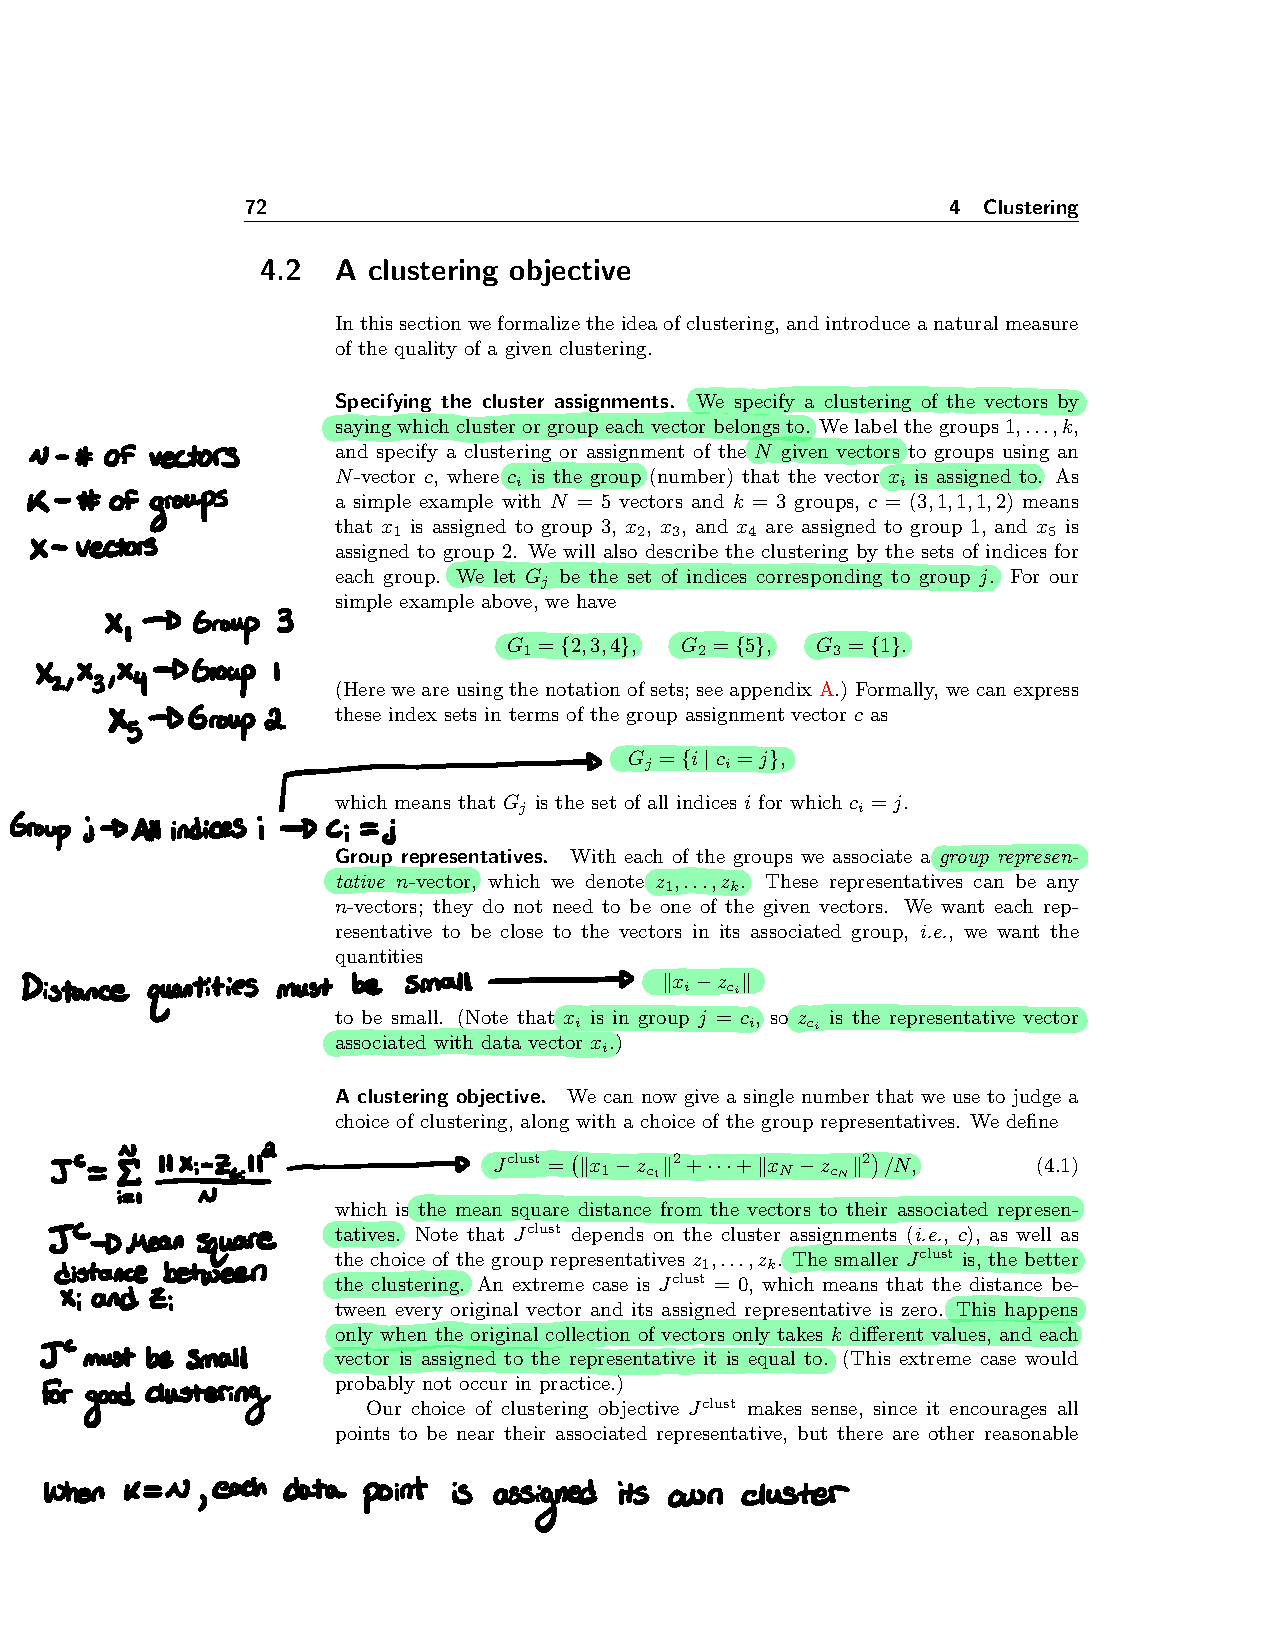
\includepdf[pages={-}, pagecommand={\thispagestyle{fancy}}, width=\paperwidth, offset=0 0]{./PDF/Annotations.pdf}
\end{problem}

% Problem 2
\begin{summary}{Problem 2 Summary}
    \begin{statement}{Procedure}
        \begin{itemize}
            \item Annotate a section from the textbook by adding comments and insights for the given section
        \end{itemize}
    \end{statement}
    \begin{statement}{Key Concepts}
        \begin{itemize}
            \item This section of the textbook covers the topic of clustering an objective
            \item Clustering involves grouping data points together based upon their similarities
            \item The lower the value of $J_{C}$ the better the clustering of data points
            \item $J_{c}$ is calculated with 
            \begin{equation*}
                J_{C} = \sum_{i = 1}^{N}\sum_{j = 1}^{k} \frac{1}{N} \mathbf{min}(\|x_{i} - z_{j}\|^{2})
            \end{equation*}
            \item The term $z_{j}$ is calculated with
            \begin{equation*}
                z_{j} = \frac{1}{|G_{j}|} \sum_{i \in G_{j}}^{n} x_{i}
            \end{equation*}
            where $G_{j}$ is group $j$ for a given data set and $|G_{j}|$ is the number of elements in that group
        \end{itemize}
    \end{statement}
    \begin{statement}{Variations}
        \begin{itemize}
            \item We could be asked to annotate a different section from the textbook
        \end{itemize}
    \end{statement}
\end{summary}

% Problem 3
\begin{problem}{Problem 3}
    \begin{statement}{Problem Statement}
        Explain example 4.4.1 in detail. Why is this an interesting example? What is $k$ in this example?
    \end{statement}

    \begin{highlight}[Solution]
        \subsubsection*{Overview}

        This example demonstrates a use of the $k$-means algorithm to cluster data that represents hand written digits. There are a total of 60,000 images in the MNIST database of handwritten images.
        Each image is an image with 784 pixels, where each pixel is represented with a value that is indicative of the brightness of the pixel in question. One can interpret each pixel to be a vector
        of length 1 (or a scalar value for that matter). The images in question are $28 \times 28$ with a total of 784 pixels. Each image is a vector of length 784.

        In the context of the $k$-means algorithm, the clustering that is done on these images is with a $k$ value of 20. This means that when the algorithm is ran, the pixels are clustered into 20
        separate clusters that are assembled to resemble a digit that was initially hand drawn. \vspace*{1em}

        \subsubsection*{Process}

        Each individual image is ran through the $k$-means algorithm with $k = 20$. The images in the example are then processed three times and there is a plot that represents each iteration of the
        algorithm for three different initial partitions of the data. Figure 4.7 has three colored lines, the line that is \textcolor{red}{red} represents the initial partition with the worst clustering
        of the data. The line that is \textcolor{blue}{blue} represents the partition that had the best clustering of the data. The \textcolor{brown}{brown} line in the graph is the partition that is
        the median valued partition of the data. \vspace*{1em}

        \begin{center}
            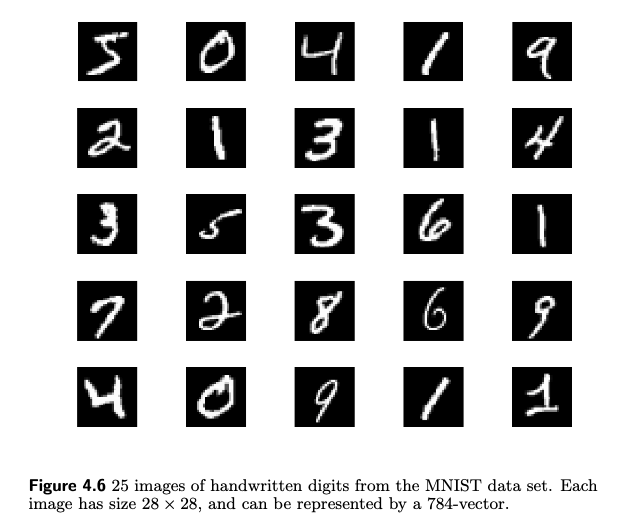
\includegraphics[width = 0.38\textwidth]{./Images/Figure 4.6.png}
            \hspace*{20pt}
            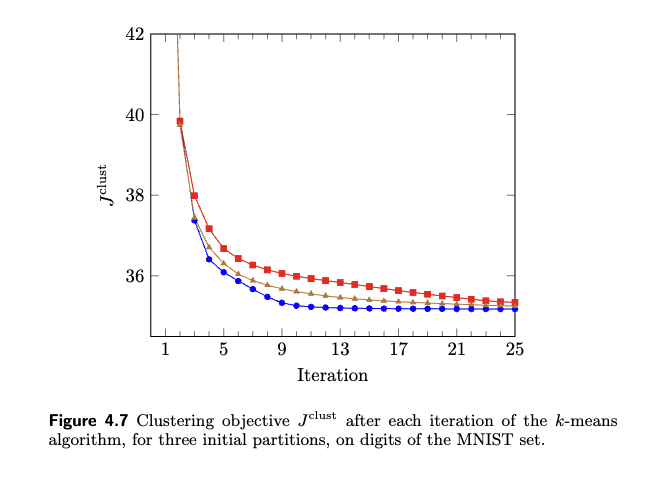
\includegraphics[width = 0.45\textwidth]{./Images/Figure 4.7.png}
        \end{center}
        Figure 4.6 represents some examples of the images found in MNIST database and Figure 4.7 represents the comparison of clustering that was done on the images with three different random partitions
        of the centroids in the $k$-means algorithm. \vspace*{1em}

        \subsubsection*{Comparison}

        Figure 4.8 below is the partition that had the worst clustering. Consequently, the digits in these are very blurry and that is indicative visually with a clustering of data that is poor. Figure 
        4.9 on the other hand is the partition that had the best clustering. Although some of the images are blurry, most of the images in this figure are easily identifiable and this is indicative of 
        better clustering. \vspace*{1em}
        
        \begin{center}
            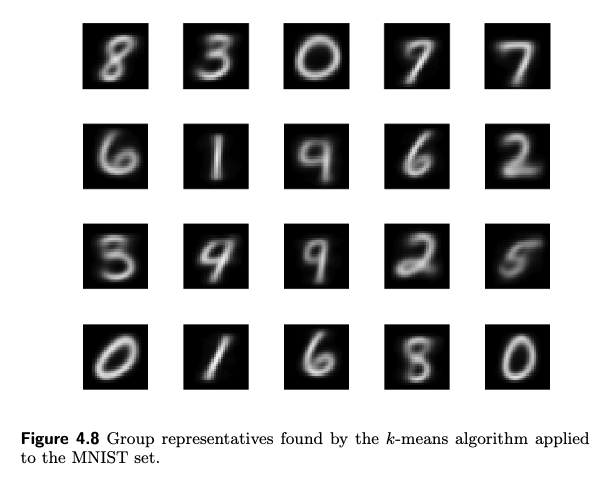
\includegraphics[width = 0.45\textwidth]{./Images/Figure 4.8.png}
            \hspace*{20pt}
            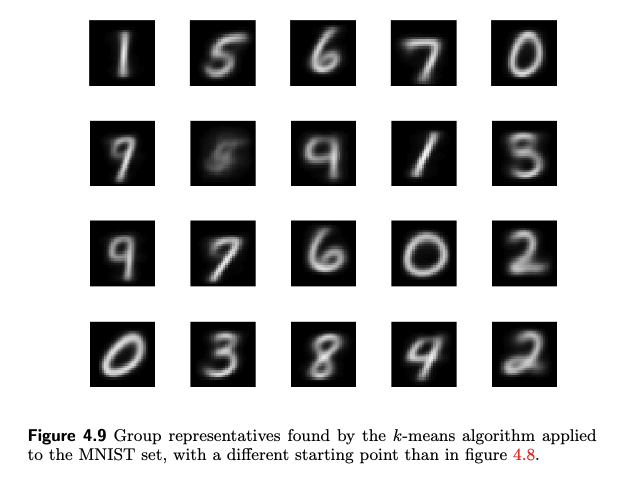
\includegraphics[width = 0.45\textwidth]{./Images/Figure 4.9.png}
        \end{center}
        The $k$-means algorithm appears to struggle with images that have the digits $4,9,3$ or $8$ in them. This is because the representation of these images can be somewhat ambiguous when trying to cluster
        the data because of the similarity of the digits with others. \vspace*{1em}

        \subsubsection*{Insights}

        This is an interesting example, because of how blurry the digits may be in some cases, the $k$-means algorithm does a pretty good job of representing digits. Since the algorithm doesn't really know
        anything about how digits look to the human eye, it does an exceptionally good job at re-creating digits regardless of how blurry they might be to us who know what these digits look like if they are
        written clearly.
    \end{highlight}
\end{problem}

% Problem 3 Summary
\begin{summary}{Problem 3 Summary}
    \begin{statement}{Procedure}
        \begin{itemize}
            \item Analyze the process of how $k$-means algorithm works for this specific example of images
        \end{itemize}
    \end{statement}
    \begin{statement}{Key Concepts}
        \begin{itemize}
            \item This problem showcases the $k$-means algorithm and how it works for a given set of images and how it can be used to re-create images with the use of clustering
            \item The $k$ value in $k$-means is the number of clusters that the algorithm is attempting to cluster data into
            \item The lower the value of $J_{C}$ the better the clustering of data
        \end{itemize}
    \end{statement}
    \begin{statement}{Variations}
        \begin{itemize}
            \item We could be given a different set of images that we would need to analyze for how the $k$-means algorithm works
            \begin{itemize}
                \item In this case we would use the same process of analyzing the images and see how the $k$-means algorithm performs in those scenarios
            \end{itemize}
        \end{itemize}
    \end{statement}
\end{summary}

% Problem 4
\begin{problem}{Problem 4}
    \begin{statement}{Problem Statement}
        Explain the solution to 4.1  here in your own words. (Since you are given a solution, you will be graded on your ability to explain).

        \subsubsection*{Original Question}

        \textit{Minimizing mean square distance to a set of vectors.} Let $x_{1}, \dots, x_{L}$ be a collection of $n$-vectors. In this exercise you will fill in the missing parts of the argument to 
        show that the vector $z$ which minimizes the sum-square distance to the vectors,

        \begin{equation*}
            J(z) = ||x_{1} - z||^{2} + \dots + ||x_{L} - z||^{2},
        \end{equation*}
        is the average or centroid of the vectors, $\bar{x} = (1/L) (x_{1} + \dots + x_{L})$. (This result is used in one of the steps in the $k$-means algorithm. But here we have simplified the notation.)

        \begin{enumerate}[label = (\alph*)]
            \item Explain why, for any $z$, we have
            \begin{equation*}
                J(z) = \sum^{L}_{i = 1} ||x_{i} - \bar{x} - (z - \bar{x})||^{2} = \sum^{L}_{i = 1} (||x_{i} - \bar{x}||^{2} - 2(x_{i} - \bar{x})^{T}(z - \bar{x}) + L||z - \bar{x}||^{2}).
            \end{equation*}
            \item Explain why $\sum^{L}_{i = 1}(x_{i} - \bar{x})^{T}(z - \bar{x}) = 0$. \textit{Hint.} Write the left-hand side as 
            \begin{equation*}
                \Bigg(\sum^{L}_{i = 1} (x_{i} - \bar{x})\Bigg)^{T}(z - \bar{x}),
            \end{equation*}
            and argue that the left-hand vector is 0.
            \item Combine the results of (a) and (b) to get $J(z) = \sum^{L}_{i = 1}||x_{i} - \bar{x}||^{2} + L||z - \bar{x}||^{2}$. Explain why for any $z \neq \bar{x}$, we have $J(z) > J(\bar{x})$. This shows
            that the choice $z = \bar{x}$ minimizes $J(z)$.
        \end{enumerate}
    \end{statement}

    \begin{highlight}[Solution - Part (a)]
        \noindent For this problem, I will be using \textbf{Method 4}.

        \subsubsection*{VMLS Solution:}

        \begin{enumerate}[label = (\alph*)]
            \item In the second expression, we are simply adding and subtracting the vector $\bar{x}$ from $x_{i} - z$, which has no effect. Expanding the norm squared gives the right-hand expression.
        \end{enumerate}

        \subsubsection*{Explanation:}

        We first begin by cleverly adding 0 the LHS of the problem statement. This is done by adding and subtract the vector $\bar{x}$. Namely,

        \setcounter{equation}{0}
        \begin{equation}
            J(z) = \sum^{L}_{i = 1} ||x_{i} - z + \bar{x} - \bar{x}||^{2} = \sum^{L}_{i = 1} ||x_{i} - \bar{x} - z + \bar{x}||^{2} = \sum^{L}_{i = 1} ||(x_{i} - \bar{x}) - (z - \bar{x})||^{2}
        \end{equation}
        where we have just regrouped the terms in equation (1) to get our final expression on the RHS. We know from VMLS that the norm of two vectors being summed is 

        \begin{equation*}
            ||\alpha + \beta||^{2} = ||\alpha||^{2} + 2\alpha^{T}\beta + ||\beta||^{2}.
        \end{equation*}
        If we then apply the definition of a norm from VMLS with the RHS of equation (1) and make the substitution of $\alpha = (x_{i} - \bar{x})$ and $\beta = (z - \bar{x})$ we then have

        \begin{equation}
            J(z) = \sum^{L}_{i = 1} ||(x_{i} - \bar{x}) - (z - \bar{x})||^{2} = \sum^{L}_{i = 1} (||x_{i} - \bar{x}||^{2} - 2(x_{i} - \bar{x})^{T}(z - \bar{x}) + L||z - \bar{x}||^{2}).
        \end{equation}
        The minus sign in equation (2) is coming from the fact that we are computing the distance and not the sum. The variable $L$ comes from scaling the difference between $z$ and $\bar{x}$.
    \end{highlight}

    \begin{highlight}[Solution - Part (b)]
        \noindent For this problem, I will be using \textbf{Method 4}.

        \subsubsection*{VMLS Solution:}

        \begin{enumerate}[label = (\alph*), start = 2]
            \item We follow the hint, which works since the inner product is a linear function, so
            
            \begin{equation*}
                \sum^{L}_{i = 1} (x_{i} - \bar{x})^{T}(z - \bar{x}) = \Bigg(\sum^{L}_{i = 1} (x_{i} - \bar{x})\Bigg)^{T}(z - \bar{x})
            \end{equation*}
            (Note that the first sum is over numbers, and the second is over vectors.) Note also that the right-hand vector in the inner product is the same for each $i$. The vector 
            $\sum^{L}_{i = 1}(x_{i} - \bar{x})$ is zero, since
            
            \begin{equation*}
                \sum^{L}_{i = 1} x_{i} = L \bar{x} = \sum^{L}_{i = 1} \bar{x}.
            \end{equation*}
            Therefore the middle term in the right-hand expression for $J(z)$ in part (a) is zero.
        \end{enumerate}

        \subsubsection*{Explanation:}

        We know from the problem statement that $\bar{x}$ can be written as 

        \begin{equation}
            \bar{x} = \frac{1}{L}(x_{1} + \dots + x_{L}) = \frac{1}{L} \sum^{L}_{i = 1} x_{i}.
        \end{equation}
        This means if we isolate $x_{i}$ from equation (3) we can then say 

        \begin{equation}
            \sum^{L}_{i = 1}x_{i} = L \bar{x}.
        \end{equation}
        Going back to the problem statement for part (b), if we substitute equation (4) into it we have 

        \begin{equation}
            \sum^{L}_{i = 1} (x_{i} - \bar{x})^{T}(z - \bar{x}) = \sum^{L}_{i = 1} (\bar{x} - \bar{x})^{T}(z - \bar{x}) = \sum^{L}_{i = 1} (0)^{T}(z - \bar{x}) = 0
        \end{equation}
        and thus we have $\sum^{L}_{i = 1}(x_{i} - \bar{x})^{T}(z - \bar{x}) = 0$.
    \end{highlight}

    \begin{highlight}[Solution - Part (c)]
        \noindent For this problem, I will be using \textbf{Method 4}. 

        \subsubsection*{VMLS Solution:}

        \begin{enumerate}[label = (\alph*), start = 3]
            \item For any $z \neq \bar{x}$, we have
            
            \begin{equation*}
                J(z) = \sum^{L}_{i = 1}||x_{i} - \bar{x}||^{2} + L||z - \bar{x}||^{2} > \sum^{L}_{i = 1} ||x_{i} - \bar{x}||^{2} = J(\bar{x}),
            \end{equation*}
            where we use $||z - \bar{x}|| > 0$.
        \end{enumerate}

        \subsubsection*{Explanation:}

        We know from part (b) that the term 

        \begin{equation}
            \sum^{L}_{i = 1} (x_{i} - \bar{x})^{T} = 0.
        \end{equation}
        Substituting equation (6) into equation (2) we can then say 

        \begin{align}
            J(z) & = \sum^{L}_{i = 1} (||x_{i} - \bar{x}||^{2} - 2(x_{i} - \bar{x})^{T}(z - \bar{x}) + L||z - \bar{x}||^{2}) \\
            & = \sum^{L}_{i = 1} (||x_{i} - \bar{x}||^{2} - 2(0)(z - \bar{x}) + L||z - \bar{x}||^{2}) \\
            & = \sum^{L}_{i = 1} (||x_{i} - \bar{x}||^{2} + L||z - \bar{x}||^{2})
        \end{align}
        where equation (9) is the representation of $J(z)$ when $z \neq \bar{x}$. If we assume that $z = \bar{x}$ then equation (7) becomes 

        \begin{align}
            J(\bar{x}) & = \sum^{L}_{i = 1} (||x_{i} - \bar{x}||^{2} - 2(x_{i} - \bar{x})^{T}(\bar{x} - \bar{x}) + L||\bar{x} - \bar{x}||^{2}) \\
            & = \sum^{L}_{i = 1} (||x_{i} - \bar{x}||^{2} - 2(0)^{T}(0) + L||0||^{2}) \\
            & = \sum^{L}_{i = 1} ||x_{i} - \bar{x}||^{2}.
        \end{align}
        Comparing equation (9) to that of equation (12), it is obvious that because of the extra term in equation (9), we can say

        \begin{equation}
            J(z) > J(\bar{x}).
        \end{equation}
    \end{highlight}
\end{problem}

% Problem 4 Summary
\begin{summary}{Problem 4 Summary}
    \begin{statement}{Procedure}
        \begin{enumerate}[label = (\alph*)]
            \item Part (a)
            \begin{itemize}
                \item Add the term ($\bar{x} - \bar{x}$) to the original expression and carry out the algebra to get to the final expression
            \end{itemize}
            \item Part (b)
            \begin{itemize}
                \item Carry out the algebra for what the inner product will evaluate to and show that the inner product in the term is zero
            \end{itemize}
            \item Part (c)
            \begin{itemize}
                \item Carry out the algebra again with this specific scenario to arrive to the final expression
            \end{itemize}
        \end{enumerate}
    \end{statement}
    \begin{statement}{Key Concepts}
        \begin{itemize}
            \item Based off of specific scenarios, we can show that $J_{C}$ is equivalent to certain values
        \end{itemize}
    \end{statement}
    \begin{statement}{Variations}
        \begin{itemize}
            \item We can be given a different set of expressions to prove 
            \begin{itemize}
                \item We would then use the same procedures with properties and whatnot to prove the new expression
            \end{itemize}
        \end{itemize}
    \end{statement}
\end{summary}

% Problem 5
\begin{problem}{Problem 5}
    \begin{statement}{Problem Statement}
        Explain the solution to 4.2 here in your own words. (Since you are given a solution, you will be graded on your ability to explain).

        \subsubsection*{Original Question}

        \textit{k-means with nonnegative, proportions, or Boolean vectors.} Suppose that the vectors $x_{1}, \dots, x_{N}$ are clustered using $k$-means, with group representatives $z_{1}, \dots, z_{k}$.

        \begin{enumerate}[label = (\alph*)]
            \item Suppose the original vectors $x_{i}$ are nonnegative, i.e., their entries are nonnegative. Explain why the representatives $z_{j}$ are also nonnegative.
            \item Suppose the original vectors $x_{i}$ represent proportions, i.e., their entries are nonnegative and sum to one. (This is the case when $x_{i}$ are word count histograms, for example.) 
            Explain why the representatives $z_{j}$ also represent proportions, i.e., their entries are nonnegative and sum to one.
            \item Suppose the original vectors $x_{i}$ are Boolean, i.e., their entries are either 0 or 1. Give an interpretation of $(z_{j})_{i}$, the $i^{\text{th}}$ entry of the $j$ group representative.
        \end{enumerate}
        \textit{Hint.} Each representative is the average of some of the original vectors. The group representation $z_{j}$ is the average of the vectors $x_{k}$ in the group:

        \begin{equation*}
            z_{j} = \frac{1}{|G_{j}|} \sum_{k \in G_{j}} x_{k}.
        \end{equation*}
    \end{statement}

    \begin{highlight}[Solution - Part (a)]
        \noindent For this problem, I will be using \textbf{Method 4}. 

        \subsubsection*{VMLS Solution:}

        \begin{enumerate}[label = (\alph*), start = 1]
            \item If the vectors $x_{k}$ are nonnegative, the average $z_{j}$ is a nonnegative vector.
        \end{enumerate}

        \subsubsection*{Explanation:}

        With the equation for $z_{j}$, we have 
        
        \setcounter{equation}{0}
        \begin{equation}
            z_{j} = \frac{1}{|G_{j}|} \sum_{k \in G_{j}} x_{k}.
        \end{equation}
        In equation (1), since $|G_{j}|$ is nonnegative, it is impossible for $z_{j}$ to be nonnegative as long as $x_{k}$ is nonnegative. Therefore $z_{j}$ is nonnegative.
    \end{highlight}

    \begin{highlight}[Solution - Part (b)]
        \noindent For this problem, I will be using \textbf{Method 4}. 

        \subsubsection*{VMLS Solution:}

        \begin{enumerate}[label = (\alph*), start = 2]
            \item If each vector sums to one, $\mathbf{1}^{T}x_{k} = 1$ for all $k$, then the same is true for the average:
            
            \begin{equation*}
                \mathbf{1}^{T}z_{j} = \frac{1}{|G_{j}|} \sum_{k \in G_{j}} \mathbf{1}^{T}x_{k} = \frac{|G_{j}|}{|G_{j}|} = 1.
            \end{equation*}
        \end{enumerate}

        \subsubsection*{Explanation:}

        For each vector to sum to one, a vector $\alpha_{i}$ would look like

        \begin{equation}
            \mathbf{1}^{T}\alpha_{i} = 1.
        \end{equation}
        Applying equation (2) to $z_{j}$, $z_{j}$ would then look like

        \begin{equation}
            \mathbf{1}^{T}z_{j} = \frac{1}{|G_{j}|} \sum_{k \in G_{j}} \mathbf{1}^{T}x_{k}.
        \end{equation}
        According to VMLS, $|G_{j}|$ is the number of elements that belong to group $j$. This then means the term $\sum_{k \in G_{j}} \mathbf{1}^{T}x_{k}$ is going to have the same number of elements
        as group $j$. In turn, this means we can simplify equation (3) to now be

        \begin{equation}
            \mathbf{1}^{T}z_{j} = \frac{1}{|G_{j}|} \sum_{k \in G_{j}} \mathbf{1}^{T}x_{k} = \frac{|G_{j}|}{|G_{j}|} = 1.
        \end{equation}
        $z_{j}$ represents the proportions because the entries are nonnegative and sum to one.
    \end{highlight}

    \begin{highlight}[Solution - Part (c)]
        \noindent For this problem, I will be using \textbf{Method 4}. 

        \subsubsection*{VMLS Solution:}

        \begin{enumerate}[label = (\alph*), start = 3]
            \item The $i^{\text{th}}$ entry of group representative $z_{j}$ is the fraction of the vectors in group $j$ that have $i^{\text{th}}$ entry one. If it is equal to one, all vectors in the group 
            have $i^{\text{th}}$ entry one. If it is close to one, most vectors in the group have $i^{\text{th}}$ entry one. If it is zero, no vectors in the group have $i^{\text{th}}$ entry one.
        \end{enumerate}

        \subsubsection*{Explanation:}

        If the entries are boolean, this means that the entries are either 0 or 1. If an index $i = 1$, this means for $(z_{j})_{i}$ we have 

        \begin{equation}
            (z_{j})_{i} = 1.
        \end{equation}
        If the entry is 0, namely $i = 0$, we then have

        \begin{equation}
            (z_{j})_{i} = 0.
        \end{equation}
        This means for the vectors $x_{i}$, the entries in them are either going to be 0 or 1. When you sum the vectors to get a final value, the final value is going to represent a percentage of what vectors
        are 0 or 1. Essentially, $z_{j}$ then represents what fraction of the individual vectors $x_{i}$ are 1. If each individual vector $x_{i}$ is 0, then $z_{j}$ will be 0. If each individual vector $x_{i}$
        is 1, then $z_{j} = 1$.
    \end{highlight}
\end{problem}

% Problem 5 Summary
\begin{summary}{Problem 5 Summary}
    \begin{statement}{Procedure}
        \begin{enumerate}[label = (\alph*)]
            \item Part (a)
            \begin{itemize}
                \item Reason that the value cannot be nonnegative due to the properties of the sum
            \end{itemize}
            \item Part (b)
            \begin{itemize}
                \item Reason that the value is essentially the number of elements in a group divided by the number of elements in a group
            \end{itemize}
            \item Part (c)
            \begin{itemize}
                \item Show what it means for a boolean vector and how it applies to this scenario
            \end{itemize}
        \end{enumerate}
    \end{statement}
    \begin{statement}{Key Concepts}
        \begin{itemize}
            \item For a given set of vectors that are to be used in a $k$-means algorithm, there are specific conclusions that can be drawn from that specific example
        \end{itemize}
    \end{statement}
    \begin{statement}{Variations}
        \begin{itemize}
            \item We could be given a different set of expressions to prove
            \begin{itemize}
                \item This would require us to use properties from the given specific
            \end{itemize}
        \end{itemize}
    \end{statement}
\end{summary}